% standalone document border convention: {left bottom right top}
\documentclass[varwidth=357pt,border={0pt, -2pt, 1pt, -10pt}]{standalone}
\usepackage[force]{feynmp-auto}		    
\usepackage{amsmath}
\usepackage{graphicx}

\begin{document}
\begin{flalign*}
	P_{12} &=\hspace*{-0.5ex}
	\raisebox{-0.15ex}{
	\scalebox{0.75}{$
			\begin{gathered}
				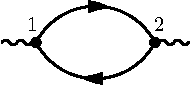
\includegraphics{polarization/poln0.pdf}
			\end{gathered}
		$}
	}
	\hspace*{-0.5ex}+\hspace*{-0.5ex}
	\raisebox{-0.15ex}{
	\scalebox{0.75}{$
			\begin{gathered}
				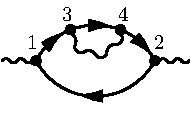
\includegraphics{polarization/poln1b.pdf}
			\end{gathered}
		$}
	}
	\hspace*{-0.5ex}+\hspace*{-0.5ex}
	\raisebox{-0.15ex}{
	\scalebox{0.75}{$
			\begin{gathered}
				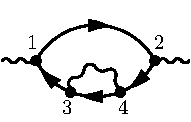
\includegraphics{polarization/poln1c.pdf}
			\end{gathered}
		$}
	}
	\hspace*{-0.5ex}+\hspace*{-0.5ex}
	\raisebox{-0.15ex}{
	\scalebox{0.75}{$
			\begin{gathered}
				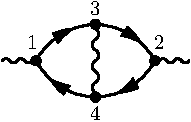
\includegraphics{polarization/poln1a.pdf}
			\end{gathered}
		$}
	}
	\\[-1ex]
	&\hspace*{3ex}+\hspace*{-0.5ex}
	\raisebox{-0.15ex}{
	\scalebox{0.75}{$
			\begin{gathered}
				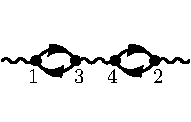
\includegraphics{polarization/poln1d.pdf}
			\end{gathered}
		$}
	}
	\hspace*{-0.5ex}+\hspace*{-0.5ex}
	\raisebox{-0.15ex}{
	\scalebox{0.75}{$
			\begin{gathered}
				
\includegraphics{polarization/poln2a.pdf}
			\end{gathered}
		$}
	}
	\hspace*{-0.5ex}+\hspace*{-0.5ex}
	\raisebox{-0.15ex}{
	\scalebox{0.75}{$
			\begin{gathered}
				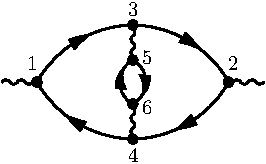
\includegraphics{polarization/poln2b.pdf}
			\end{gathered}
		$}
	}
	\hspace*{-0.5ex}+ \cdots
\end{flalign*}
\end{document}
